\documentclass{ctexart}
\usepackage[utf8]{inputenc}
\usepackage{graphicx}
\usepackage{tikz}
\usetikzlibrary{shapes,arrows}


\title{作业1: DoubleLinkedList}
\author{陈科辉 Keiver Pabula}
\date{07Octobe,2022}
\begin{document}
\maketitle

作业1:阅读课本第 91 页的 3.5, 完成模板类:DoubleLinkedList<DT>, 实现课本中 list 的全部功能;并设置外部函数find。
\section{设计思路}
根据书的代码建立双链表\\
1. 创建相应的头文件\\
2. 设计所需要的类(包括内部的大小,指针,头节点,尾节点,…)\\
3. 运算符重载\\
4. 确定所需的函数并将其设计出来,(insert, pop, printList,pushback,…)\\
5. 写出所需要的成员\\
6. 测试所需的函数\\
7. 写出所要求的外部函数\\
8. 根据要求写出主函数\\
9. debuging测试\\
10. 得到结果\\


\section{测试说明}
输出的内容\\
\begin{center}
  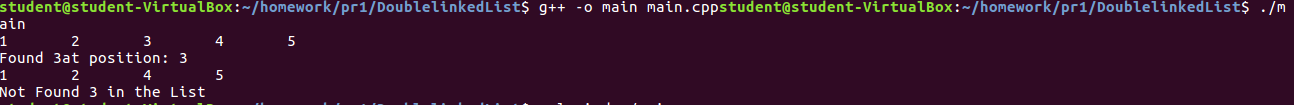
\includegraphics[scale=0.5]{1.png}
\end{center}

检查内存泄漏
\begin{center}
  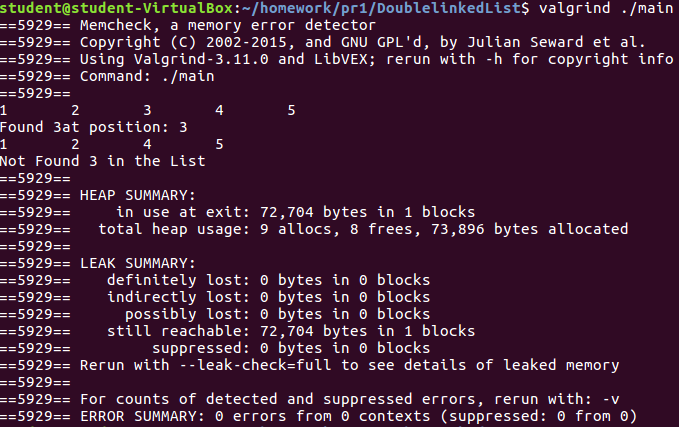
\includegraphics[scale=0.5]{2.png}
\end{center}
no leak are possible 所以无内存泄漏

\end{document}
